\documentclass[a4paper,12pt]{article}

\usepackage[portuges]{babel}
\usepackage[utf8]{inputenc}
\usepackage[T1]{fontenc}
\usepackage{lmodern}

\usepackage{amsmath, amsfonts, amssymb, array}

\usepackage{pgf, caption}
\usepackage{subcaption}

\usepackage{enumitem}

\usepackage[section]{placeins}

\usepackage{float}

%
% Page display
\addtolength{\oddsidemargin}{-0.5in}
\addtolength{\evensidemargin}{-0.5in}
\addtolength{\textwidth}{1in}

\addtolength{\topmargin}{-0.5in}
\addtolength{\textheight}{1in}

\usepackage{setspace}
\onehalfspacing

\begin{document}
	
\pagenumbering{gobble}

\vspace*{-1in}
\begin{center}
		
	\textbf{\normalsize Universidade Federal do Rio de Janeiro} \\
	\textbf{\small Instituto de Matemática} \\
	\textbf{\small Departamento de Matemática Aplicada} \\
	
	\vspace{1.5in}
	
	\doublespacing
	\textit{\textbf{\LARGE Relatório Final PIBIC -}} \\
	\textbf{\LARGE Modelagem de Dados Epidemiológicos por Equações Diferenciais Ordinárias Universais}
	
	\vspace{1.5in}
	
	\onehalfspacing
	\textbf{\Large Luan Lima Freitas} \\
	{\normalsize Aluno do Bacharelado em Matemática Aplicada - UFRJ} \\
	{\normalsize Bolsista PIBIC (04/2022 - 08/2022)} \\
	
	\vspace{0.5in}
	\textit{\large Orientador:} \\
	\textbf{\Large Prof. Dr. Ricardo Rosa} \\
	{\normalsize Departamento de Matemática Aplicada - IM/UFRJ}
\end{center}

\newpage
\pagenumbering{arabic}

\tableofcontents
\newpage

\section{Introdução}

Na vigência da bolsa de iniciação científica PIBIC (04/2022 - 08/2022), o aluno bolsista desenvolveu modelos e previsões para os dados da pandemia de COVID-19 na cidade do Rio de Janeiro, dando continuidade ao trabalho realizado durante a vigência da bolsa de iniciação científica INCTMat  (10/2021 - 02/2022). Os modelos trabalhados consistiram de equações diferenciais ordinárias universais (UODEs) [1]. As UODEs se encontram no escopo do aprendizado científico de máquina (SciML), realizando a proposta de mesclar técnicas clássicas de modelagem matemática com recursos de aprendizado de máquina. Toda a parte computacional foi implementada no ecossistema de SciML da linguagem Julia. Este trabalho dá sequência às produções dos estudantes Gil Miranda [2] e Beatriz Farah [3] sob a orientação do professor Ricardo Rosa.

\section{Equações Diferenciais Ordinárias Universais}

Avanços recentes na área de aprendizado de máquina viabilizaram a utilização de técnicas de deep learning para a modelagem de fenômenos dos quais dispõe-se de grandes quantidades de dados. Uma vantagem desta abordagem é o aprendizado automático do conjunto de interações não-lineares, as quais podem ser
tão complexas quanto numerosas. Por outro lado, esta estratégia é impraticável para a solução de problemas nos quais a disponibilidade de dados é exígua.

No extremo oposto do espectro encontram-se os modelos de equações diferenciais conhecidos como mecanicistas, na medida em que correspondem a uma tradução de fenômenos naturais (ou sociais) em um conjunto de leis explícitas, as quais representam a ação de mecanismos e exprimem um conhecimento consolidado pela literatura científica.

No intuito de conjugar as virtudes e mitigar as limitações de ambos os extremos surgem diversos modelos e métodos híbridos, dentre os quais estão as equações diferenciais ordinárias universais (UODEs), objeto do presente trabalho. Uma UODE é uma equação diferencial ordinária definida por

$$ \mathbf{u}'(t) = f(\mathbf{u}, t, U_{\boldsymbol{\theta}}(\mathbf{u},t)), $$
onde $U_{\boldsymbol{\theta}}$ é um aproximador universal, i.e., uma função capaz de aproximar qualquer função suficientemente regular. No nosso caso, o aproximador universal será dado por uma rede neural de vetor de pesos $\boldsymbol{\theta}$ que denotaremos por $N\!N_{\boldsymbol{\theta}}$. A ideia por trás de uma UODE consiste em inscrever em uma estrutura a priori legada pela experiência científica um ou mais termos capazes de adquirir dos dados relações não-lineares potencialmente intrincadas e obscuras. Uma classe particular de UODE é formada pelas equações diferenciais ordinárias neurais (NODEs) [4]. Uma NODE é uma UODE dada por
$$ \mathbf{u}'(t) = N\!N_{\boldsymbol{\theta}}(\mathbf{u}, t). $$

\section{Dados e Modelos}

Os dados disponibilizados na internet pela Secretaria Municipal de Saúde da Prefeitura do Rio de Janeiro foram manipulados para a obtenção das curvas de casos ativos, recuperados e mortos durante a pandemia de COVID-19 na cidade. Em seguida, foi selecionado um período correspondente a uma “onda” da pandemia para ser modelado por meio das técnicas mencionadas acima, qual seja, o período de 18/03/2020 a 30/06/2020 (cf. \textbf{Figura 1}).
\vspace{0.05in}

\begin{figure}[h]
	\centering
	
	\begin{subfigure}{.5\textwidth}
		\centering
		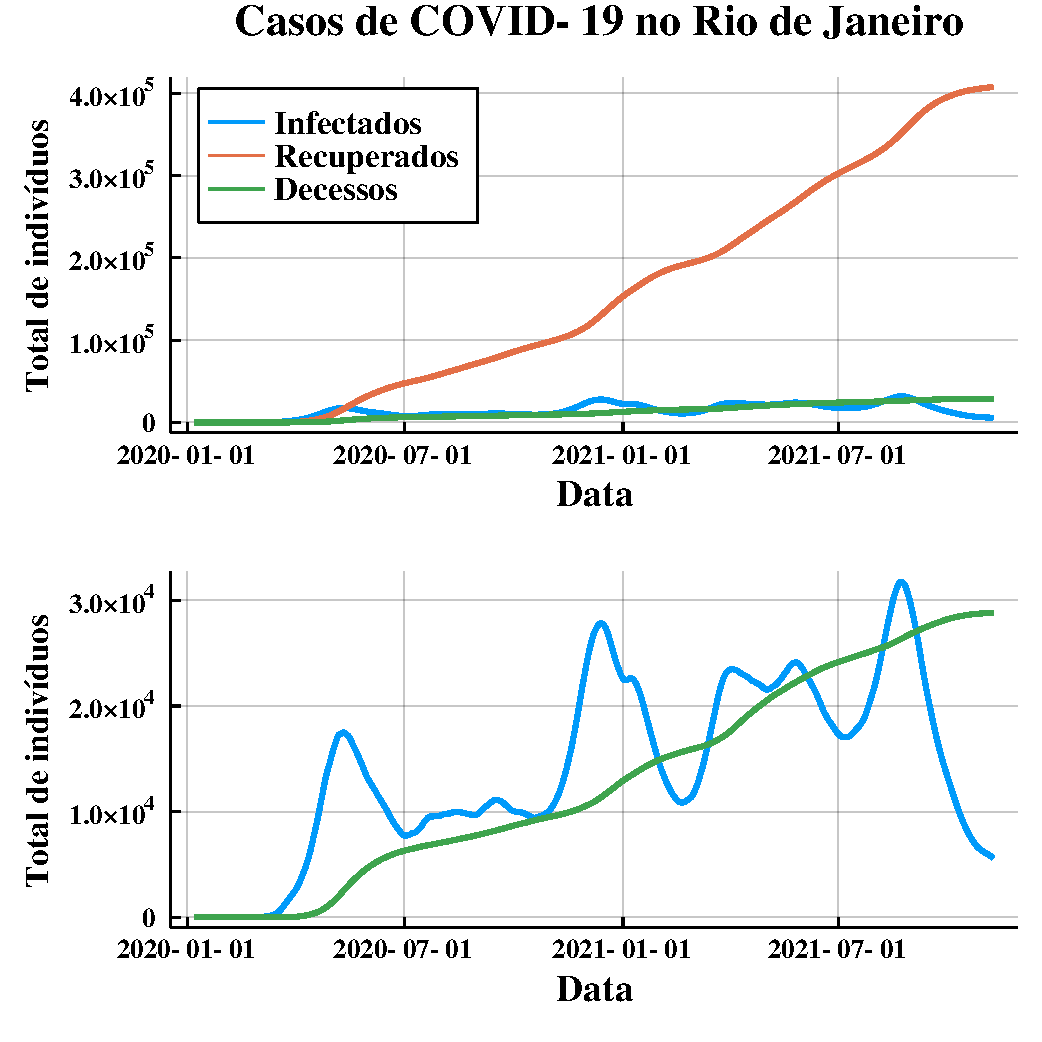
\includegraphics[width=.85\linewidth]{covid_cases}
	\end{subfigure}%
	\begin{subfigure}{.5\textwidth}
		\centering
		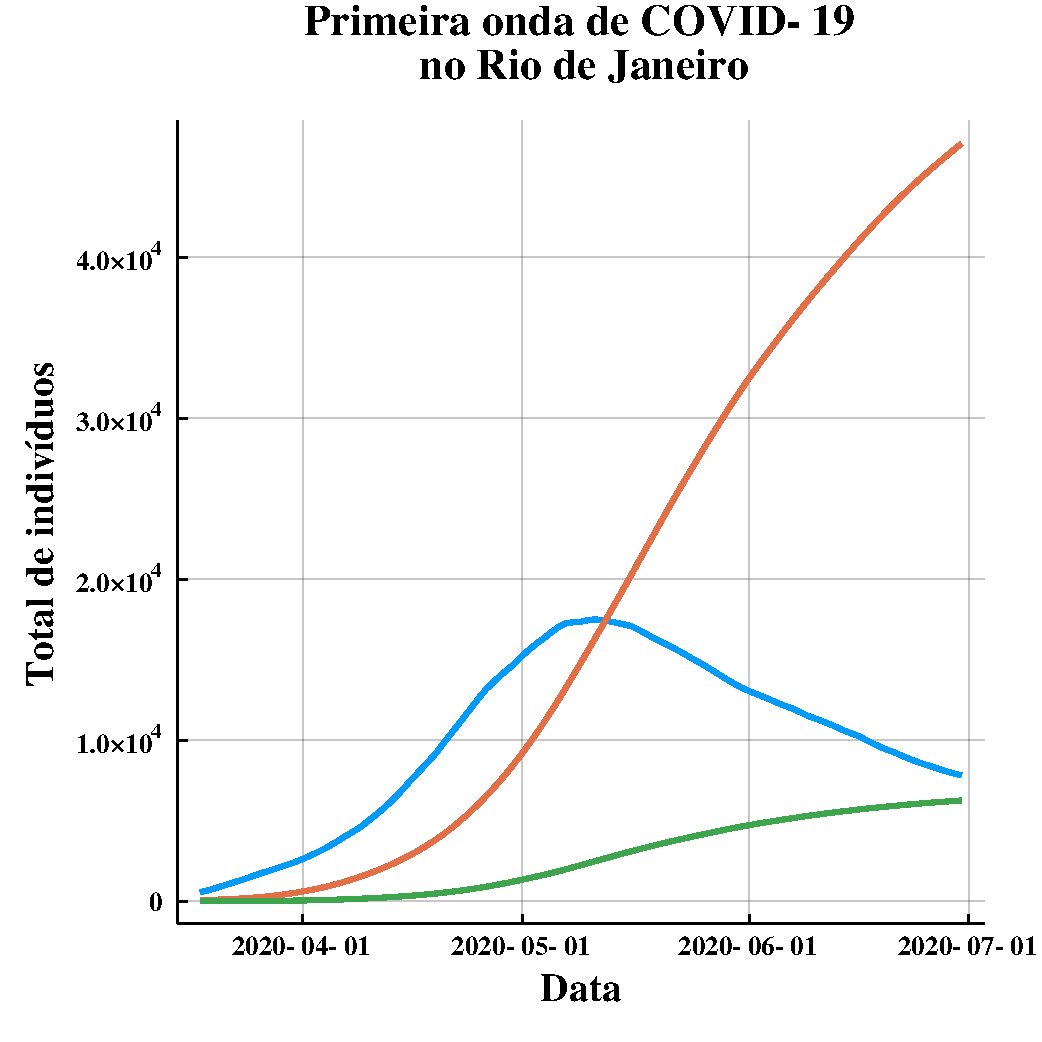
\includegraphics[width=.85\linewidth]{covid_wave}
	\end{subfigure}

	\caption*{\textbf{Figura 1:} Média móvel dos casos de COVID-19 na cidade do Rio de Janeiro.}
\end{figure}

Foi tomado como base dos experimentos o modelo compartimental SIRD. O modelo SIRD apresenta quatro compartimentos (S = “suscetíveis”, I = “infectados”, R = “recuperados” e D = “decessos”) e a evolução do número de casos em cada compartimento é dada pelo sistema de equações

$$
\left\{
\begin{array}{ccl}
	\dot S & = & -\beta \frac{I}{N} S \\
	\dot I & = &  \beta \frac{I}{N} S - \left(\gamma_R + \gamma_D\right) I\\
	\dot R & = & \gamma_R I \\
	\dot D & = & \gamma_D I
\end{array}
\right.
$$
onde $N = S+I+R+D$ e $\{\beta, \gamma_I, \gamma_R\} \subset [0, +\infty)$.

Tipicamente, a dinâmica mais árdua de se modelar em uma pandemia é a conversão dos indivíduos suscetíveis em infectados mediante a interação entre os dois grupos, no nosso caso representada pelo \textit{termo de infecção} $\beta\frac{I}{N}S$. As demais dinâmicas podem muito satisfatoriamente ser modeladas por termos lineares, havendo inclusive em alguns casos a possibilidade de estimar seus respectivos parâmetros por meio de investigações empíricas suplementares. Desta feita, propomos substituir inteira ou parcialmente o termo de infecção do modelo por redes neurais, dando assim gênese a UODEs. No nosso estudo foram contempladas duas possibilidades:

\begin{itemize}
	\item Substituir o termo de infecção por $N\!N_{\boldsymbol{\theta}}(S/N, I)$. A UODE assim definida foi nomeada de SIRD UODE $\beta$SI, onde a terminação $\beta$SI denota o termo substituído por uma rede neural.
	\item Substituir o termo de infecção por $N\!N_{\boldsymbol{\theta}}(S,I,R,D)\frac{I}{N}S$. A UODE assim definida foi nomeada de SIRD UODE $\beta$, por motivo análogo ao especificado acima.
\end{itemize}

\section{Ajuste}

Os parâmetros dos modelos definidos acima foram ajustados aos dados coletados. Sejam $I_i, R_i$ e $D_i$ os números de infectados, recuperados e decessos, respectivamente, no dia $i$. Além disso, fixada uma UODE $U$ e dado um vetor de parâmetros para $U$ $\mathbf{p}$, sejam $I_i(\mathbf{p}), R_i(\mathbf{p})$ e $D_i(\mathbf{p})$ os números de infectados, recuperados e decessos, respectivamente, determinados por $U$ e $\mathbf{p}$ no dia $i$. Os ajustes foram realizados minimizando-se a função objetivo

$$ f_1(\mathbf{p}) = \sum\limits_{i=1}^{40} \left[(I_i(\mathbf{p})- I_i)^2 + (R_i(\mathbf{p})-R_i)^2 + (D_i(\mathbf{p})-D_i)^2\right] $$
através de um método de busca por mínimos locais para diferentes valores iniciais de $\mathbf{p}$. Observou-se que o modelos ajustados diferiram significativamente para valorores iniciais de $\mathbf{p}$ diferentes. Os resultados do processo de otimização são reproduzidos abaixo, destacando-se o modelo ajustado para o qual a função objetivo atingiu seu menor valor (cf. \textbf{Figura 2}). Após o intervalo inicial de dias dedicado ao ajuste do modelo, é possível observar como cada modelo ajustado prevê a evolução subsequente da pandemia. Para efeito de comparação, também foi reproduzido o modelo SIRD ajustado.

Levando em consideração que as figuras numéricas de cada compartimento diferem substancialmente em escala, foi realizado um novo ajuste, minimizando-se uma função objetivo com pesos para cada compartimento dada por

$$ f_2(\mathbf{p}) = \frac{\sum\limits_{i=1}^{40} (I_i(\mathbf{p})- I_i)^2}{\max\limits_{i=1,\dots,40} I_i} + \frac{\sum\limits_{i=1}^{40} (R_i(\mathbf{p})- R_i)^2}{\max\limits_{i=1,\dots,40} R_i} + \frac{\sum\limits_{i=1}^{40} (D_i(\mathbf{p})- D_i)^2}{\max\limits_{i=1,\dots,40} D_i} $$

\begin{figure}[h]
	\centering
	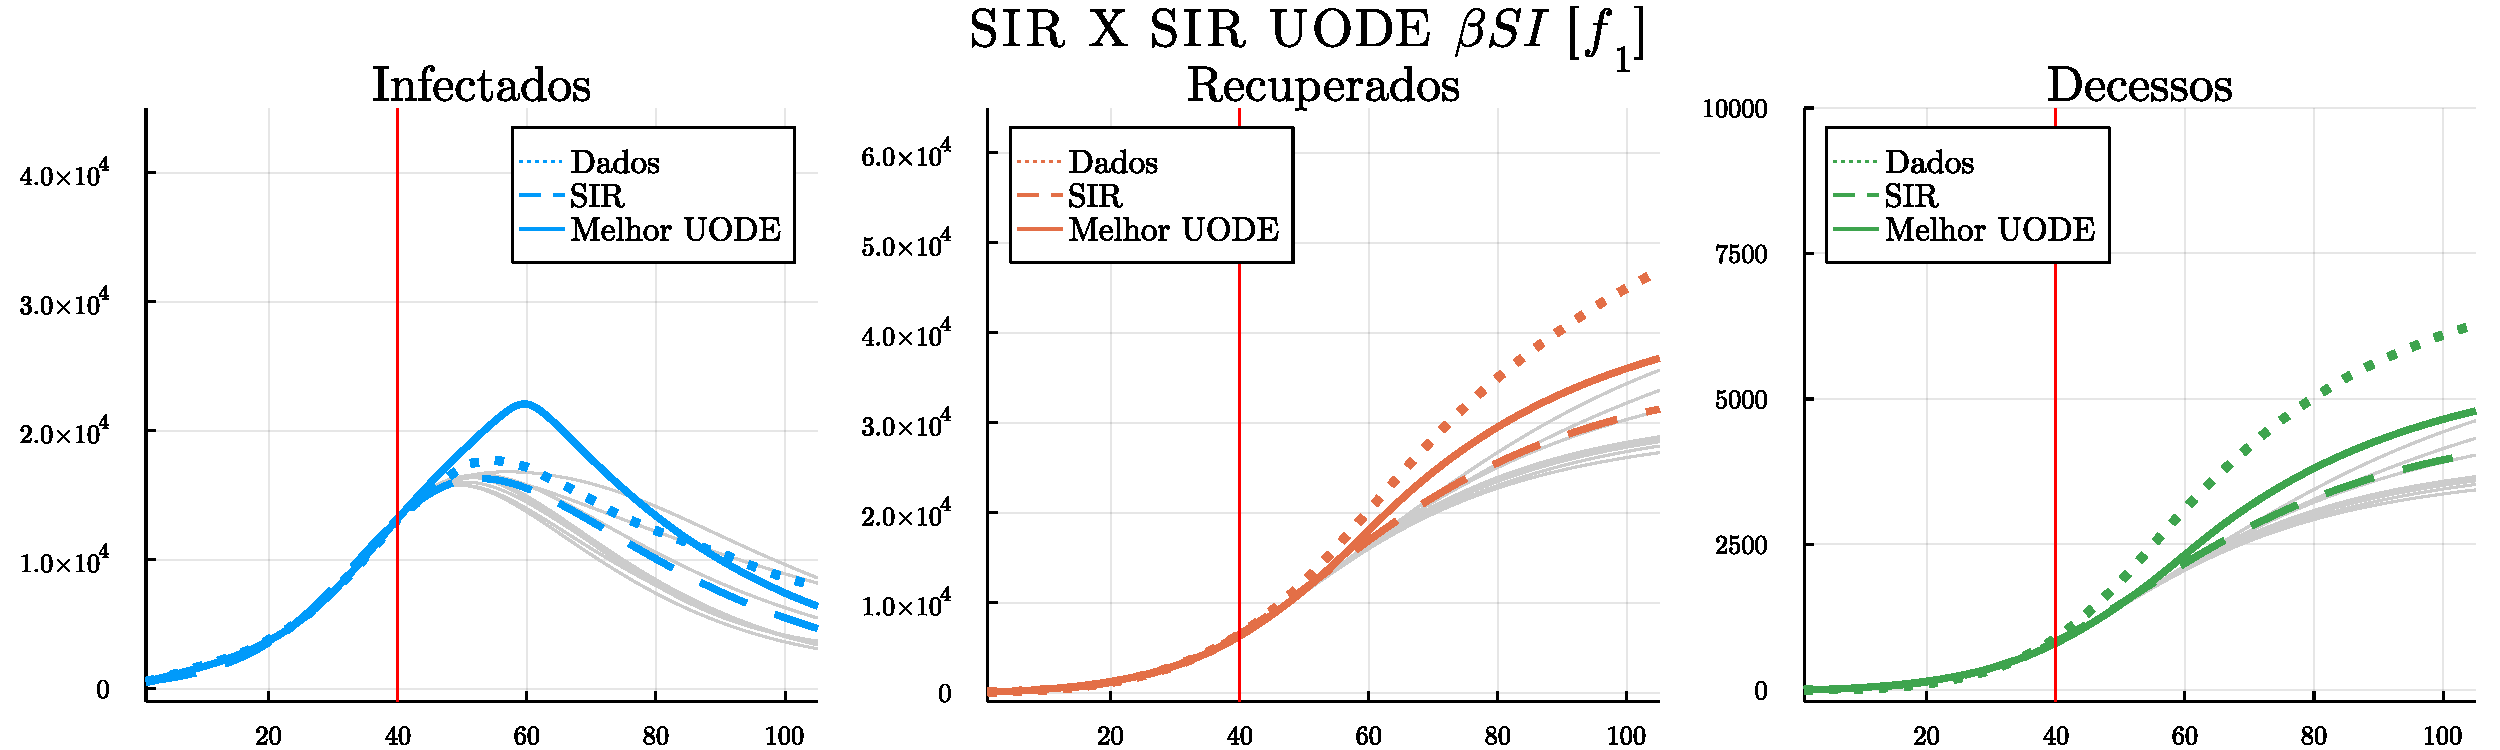
\includegraphics[width=1\textwidth]{fit1.pdf}
	\par\vspace{0.1in}
	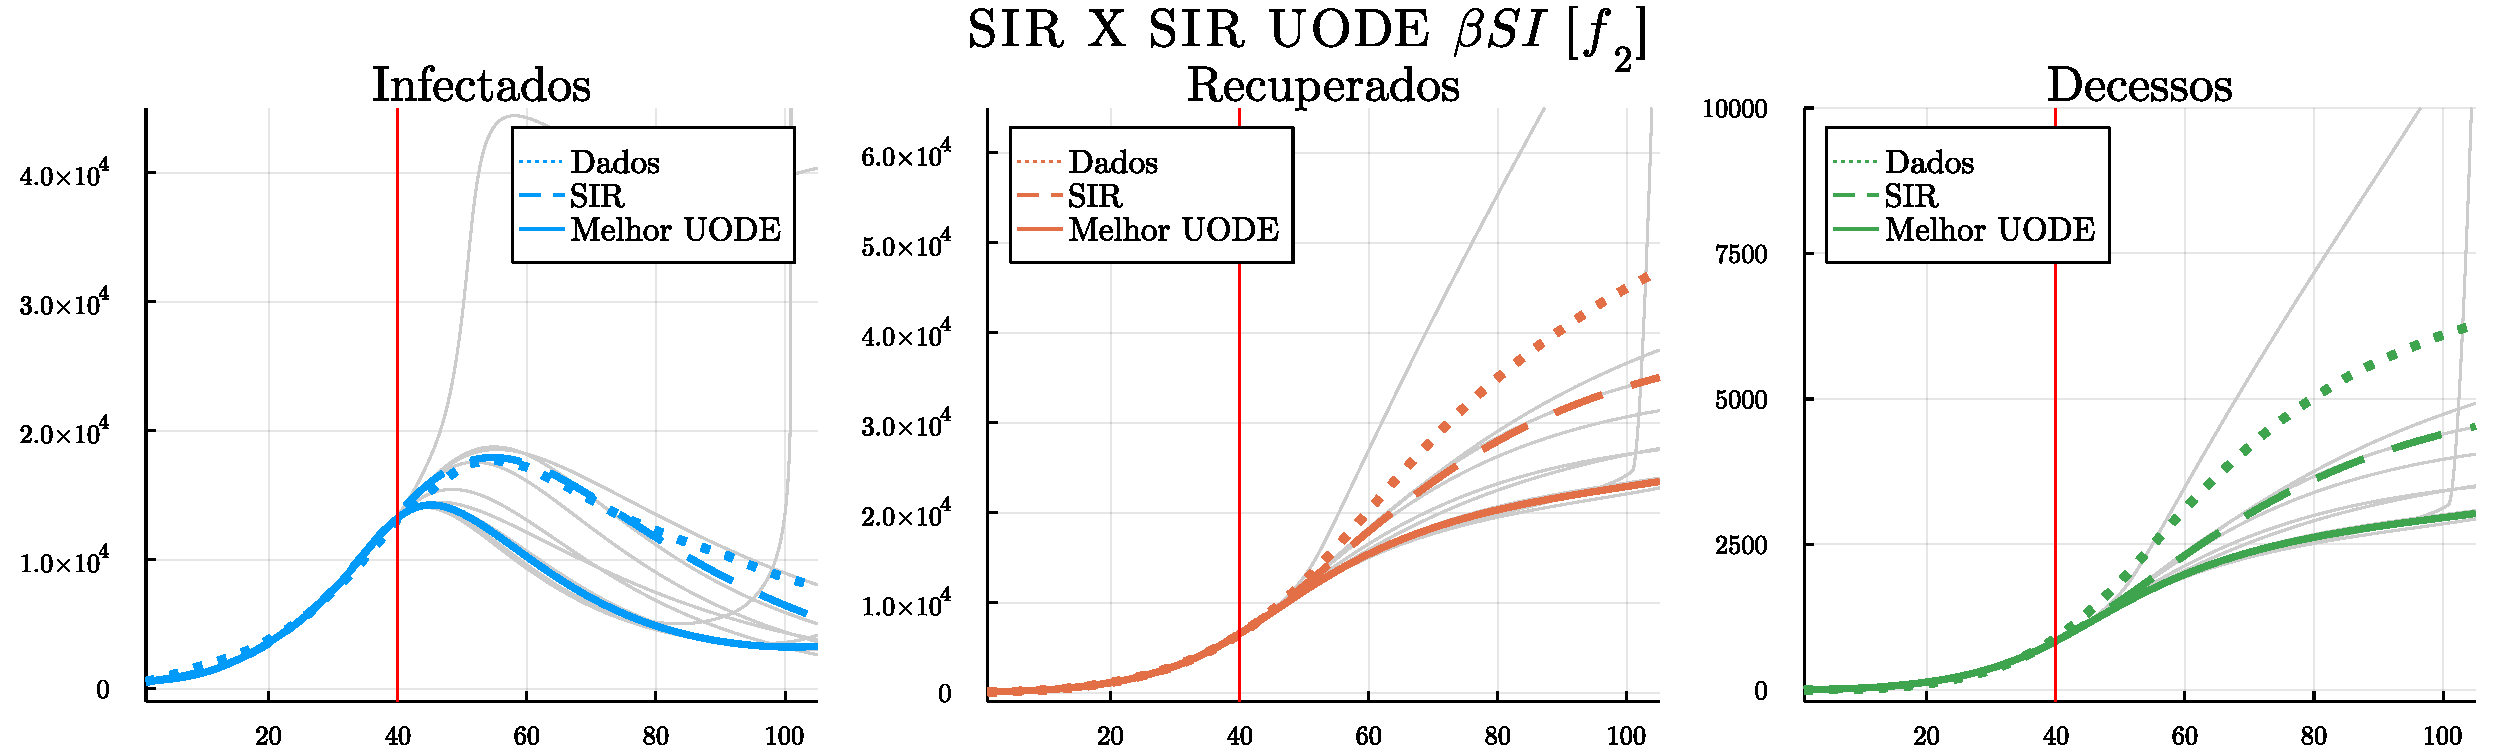
\includegraphics[width=1\textwidth]{fit2.pdf}
	\par\vspace{0.1in}
	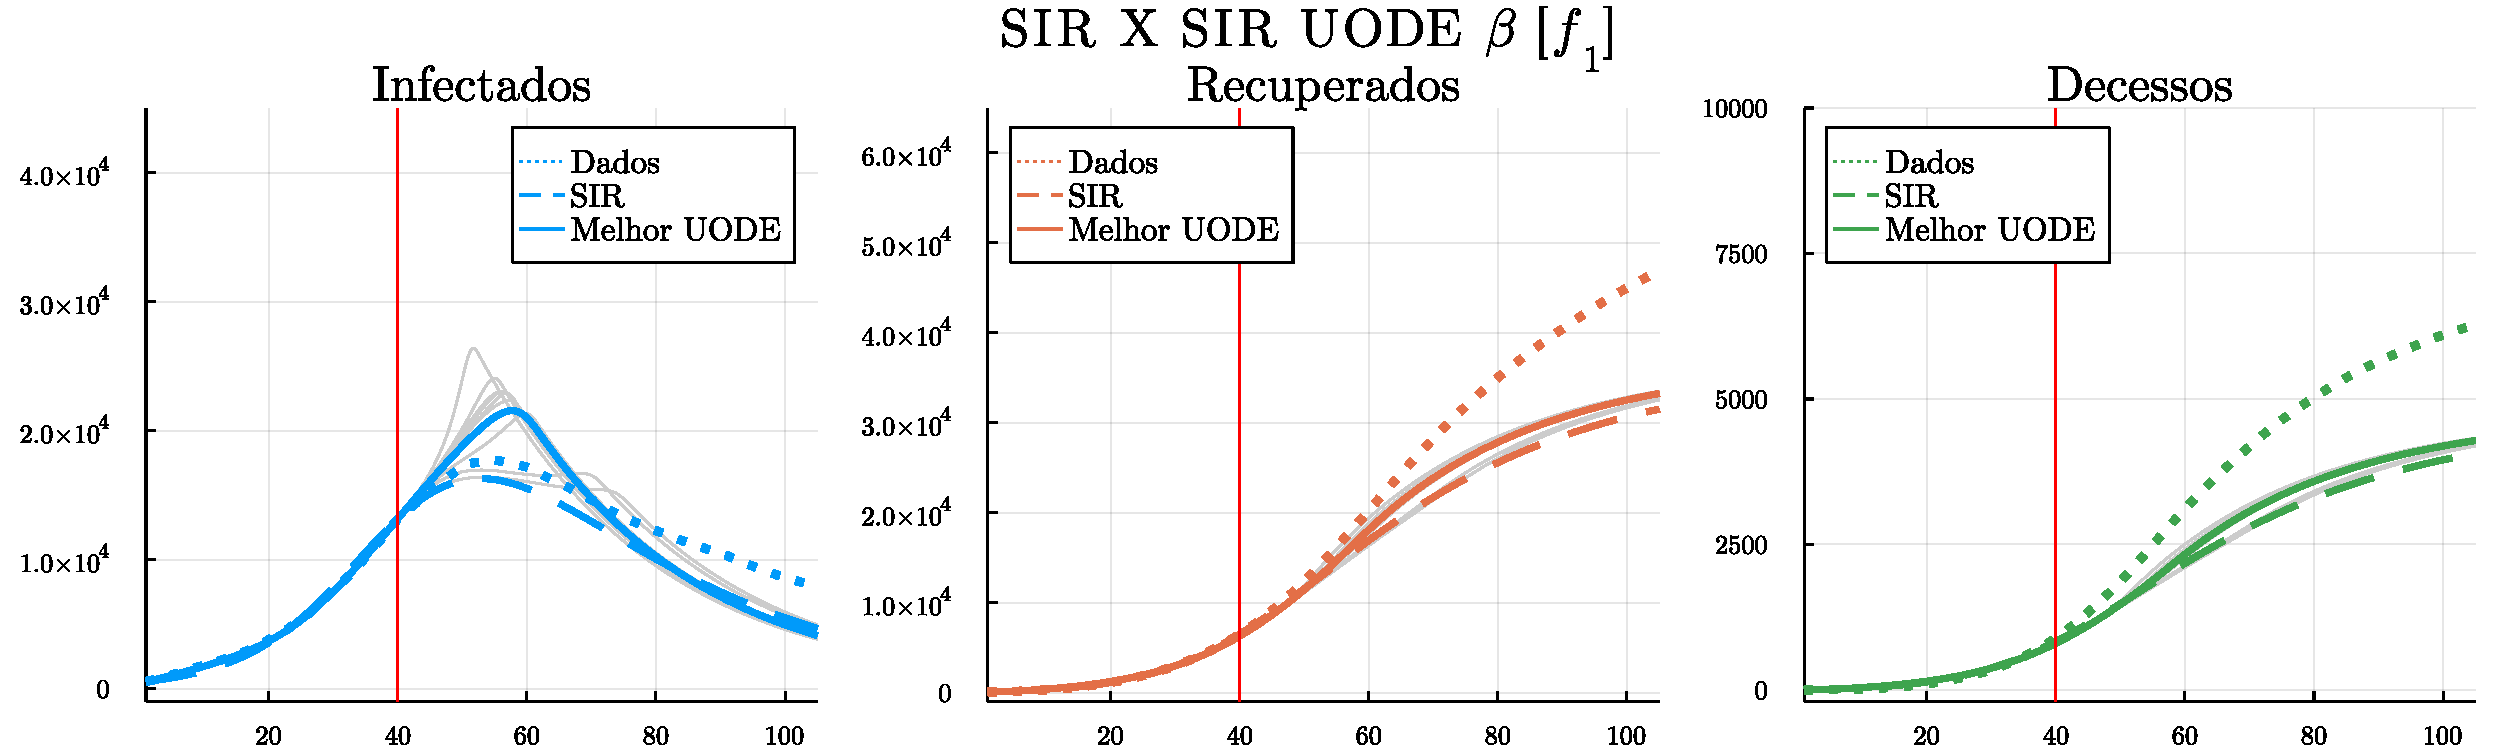
\includegraphics[width=1\textwidth]{fit3.pdf}
	\par\vspace{0.1in}
	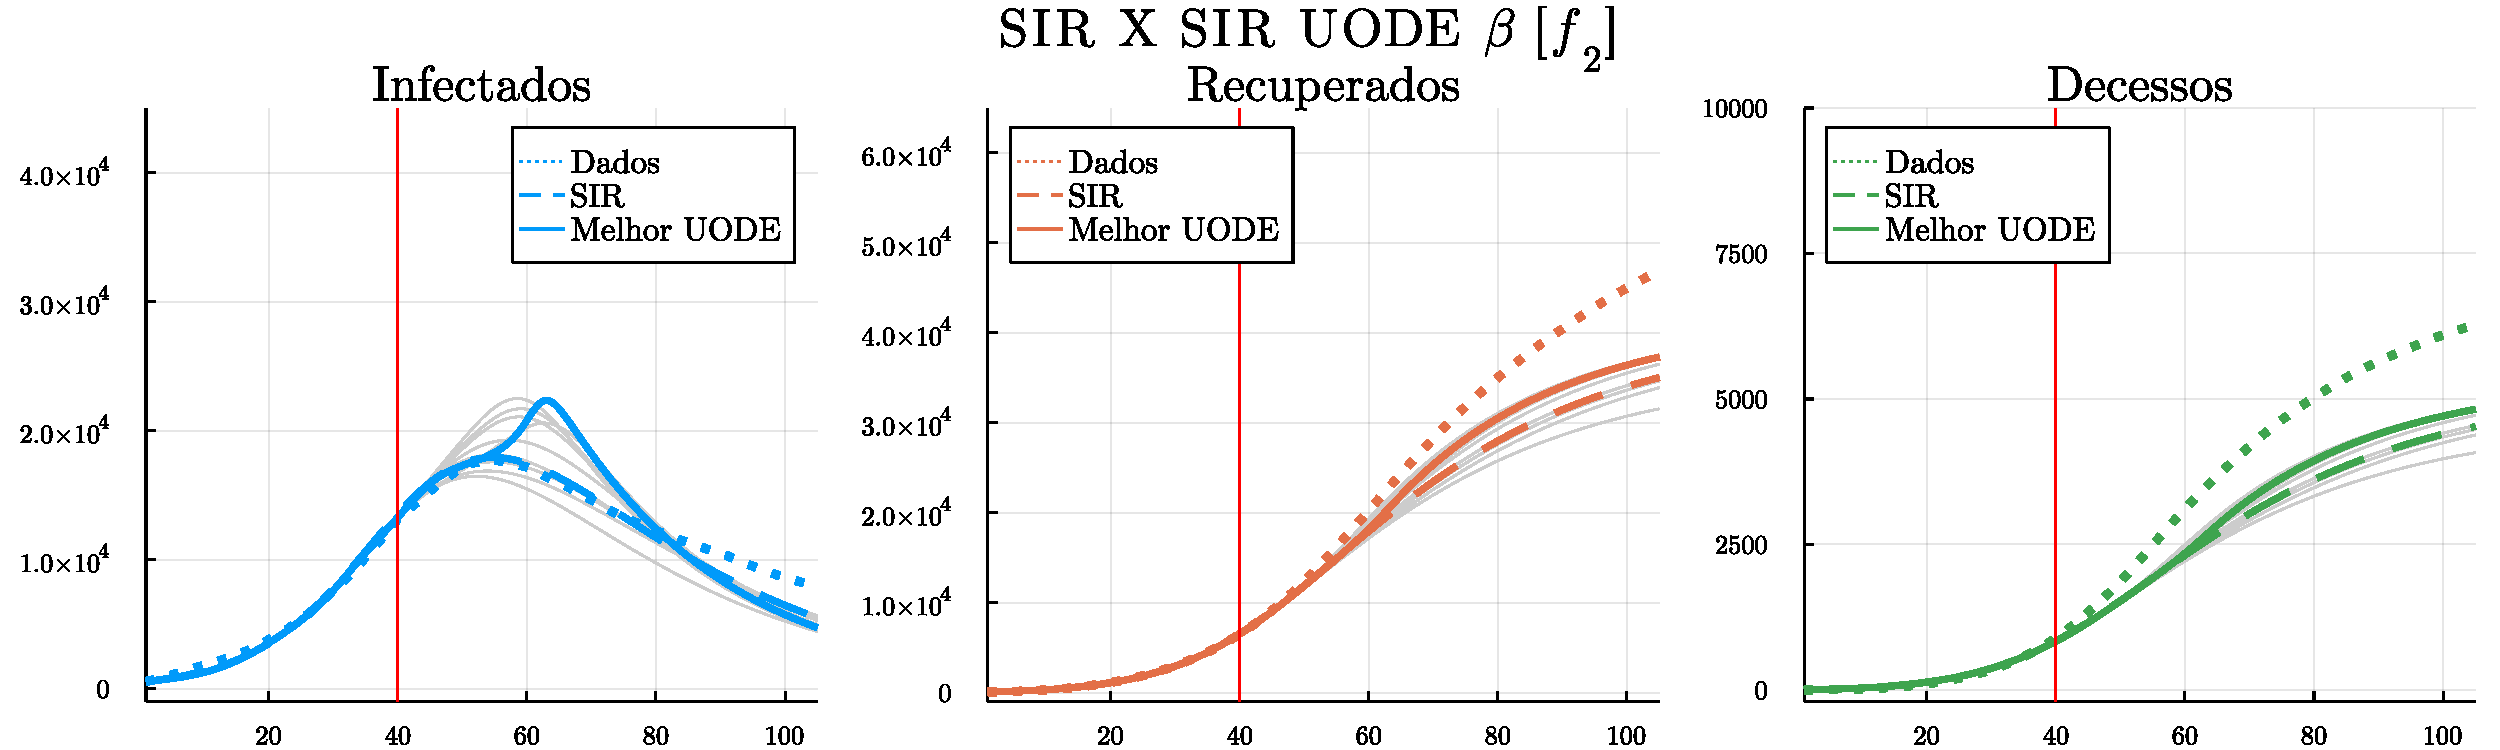
\includegraphics[width=1\textwidth]{fit4.pdf}
	
	\caption*{\textbf{Figura 1:} Média móvel dos casos de COVID-19 na cidade do Rio de Janeiro. Média móvel dos casos de COVID-19 na cidade do Rio de Janeiro. Média móvel dos casos de COVID-19 na cidade do Rio de Janeiro. Média móvel dos casos de COVID-19 na cidade do Rio de Janeiro.}
\end{figure}


\section{Referências}

\begin{enumerate}[label={[\arabic*]}]
	\item https://landscan.ornl.gov
	\item https://github.com/ModSiming/EpiSiming
\end{enumerate}

\end{document}